%particles
\newcommand{\jpsi}{\rm J/$\psi$}
\newcommand{\psip}{$\psi^\prime$}
\newcommand{\jpsiDY}{\rm J/$\psi$\,/\,DY}
\newcommand{\chic}{$\chi_{\rm c}$}
\newcommand{\pip}{$\pi^{+}$}
\newcommand{\pim}{$\pi^{-}$}
\newcommand{\pizero}{$\pi^{0}$}
\newcommand{\kap}{K$^{+}$}
\newcommand{\kam}{K$^{-}$}
\newcommand{\pbar}{$\rm\overline{p}$}
\newcommand{\ccbar}{\ensuremath{\mathrm{c\overline{c}}}}
\newcommand{\bbbar}{\ensuremath{\mathrm{b\overline{b}}}}
\newcommand{\Dzero}{\ensuremath{\mathrm{D^{0}}}}
\newcommand{\Dzerobar}{\ensuremath{\mathrm{\overline{D}^{0}}}}
\newcommand{\Dpm}{\ensuremath{\mathrm{D^{\pm}}}}
\newcommand{\Ds}{\ensuremath{\mathrm{D_{s}^{\pm}}}}
\newcommand{\Dstar}{\ensuremath{\mathrm{D^{*\pm}}}}

%collision systems
\newcommand{\pp}{pp}
\newcommand{\pPb}{p--Pb}
\newcommand{\PbPb}{Pb--Pb}

%detectors
\newcommand{\ezdc}{$E_{\rm ZDC}$}

%units
\newcommand{\GeVc}{GeV/$c$}
\newcommand{\GeVcsq}{GeV/$c^2$}

%others
\newcommand{\degree}{$^{\rm o}$}
\newcommand{\s}{\ensuremath{\sqrt{s}}}
\newcommand{\snn}{\ensuremath{\sqrt{s_{\rm NN}}}}
\newcommand{\y}{\ensuremath{y}}
\newcommand{\pt}{\ensuremath{p_{\rm T}}}
\newcommand{\dedx}{d$E$/d$x$}
\newcommand{\dndy}{d$N$/d$y$}
\newcommand{\dndydpt}{${\rm d}^2N/({\rm d}y {\rm d}p_{\rm t})$}
\newcommand{\zpar}{\ensuremath{z_{||}}}
\newcommand{\zpargen}{\ensuremath{z_{||}^{\mathrm{part}}}}
\newcommand{\zpardet}{\ensuremath{z_{||}^{\mathrm{det}}}}
\newcommand{\ptchjet}{\ensuremath{p_{\mathrm{T,ch\, jet}}}}
\newcommand{\ptjet}{\ensuremath{p_{\mathrm{T,jet}}}}
\newcommand{\ptchjetgen}{\ensuremath{p_{\mathrm{T,ch\,jet}}^{\mathrm{part}}}}
\newcommand{\ptchjetdet}{\ensuremath{p_{\mathrm{T,ch\,jet}}^{\mathrm{det}}}}
\newcommand{\ptd}{\ensuremath{p_{\mathrm{T,D}}}}
\newcommand{\ptdgen}{\ensuremath{p_{\mathrm{T,D}}^{\mathrm{part}}}}
\newcommand{\ptddet}{\ensuremath{p_{\mathrm{T,D}}^{\mathrm{det}}}}
\newcommand{\antikt}{anti-\ensuremath{k_{\mathrm{T}}}}
\newcommand{\Antikt}{Anti-\ensuremath{k_{\mathrm{T}}}}
\newcommand{\kt}{\ensuremath{k_{\mathrm{T}}}}
\newcommand{\pthard}{\ensuremath{p_{\mathrm{T,hard}}}}

\PassOptionsToPackage{usenames,dvipsnames}{xcolor}
\documentclass{tikzposter}
\usepackage{xcolor}
\usetikzlibrary{positioning}
\usetheme{Rays}

\usepackage{url}
\usepackage{adjustbox}
\usepackage{comment}
\usepackage{overpic}

\makeatletter
\def\title#1{\gdef\@title{\scalebox{\TP@titletextscale}{%
\begin{minipage}[t]{\linewidth}
\centering
#1
\par
\vspace{0.5em}
\end{minipage}%
}}}
\makeatother

\settitle{ \centering \vbox{
     \@titlegraphic \\[\TP@titlegraphictotitledistance] \centering
     \color{titlefgcolor} {\bfseries \Huge \@title \par}
     \vspace*{1em}
     {\huge \@author \par} \vspace*{1em} {\LARGE \@institute}
}}

\title{Exploring the charm content of jets
in \pp\ collisions with ALICE}
\author{Salvatore Aiola, on behalf of the ALICE Collaboration}
\institute{Yale University\\[0.01cm] \url{salvatore.aiola@yale.edu}\\[1cm] 
\begin{minipage}[t]{0.19\linewidth}
\hspace{1cm}
\end{minipage}
%
\begin{adjustbox}{valign=c}
\begin{minipage}[t]{0.1\linewidth}

\includegraphics[width=\linewidth]{img/qm17}
\end{minipage}
\end{adjustbox}
%
\begin{adjustbox}{valign=c}
\begin{minipage}[t]{0.5\linewidth}
February 6-11, 2017, Chicago, IL, USA
\end{minipage}
\end{adjustbox}
%
\begin{minipage}[t]{0.2\linewidth}
\hspace{1cm}
\end{minipage}
}
\makeatletter
\newcommand\insertlogoi[2][]{\def\@insertlogoi{\includegraphics[#1]{#2}}}
\newcommand\insertlogoii[2][]{\def\@insertlogoii{\includegraphics[#1]{#2}}}
\newcommand\insertlogoiii[2][]{\def\@insertlogoiii{\includegraphics[#1]{#2}}}
\newlength\LogoSep
\setlength\LogoSep{-150pt}

\insertlogoi[width=8cm]{img/yale}
\insertlogoii[width=4cm]{img/yale_text}
\insertlogoiii[width=7cm]{img/alice}

\renewcommand\maketitle[1][]{  % #1 keys
    \normalsize
    \setkeys{title}{#1}
    % Title dummy to get title height
    \node[transparent,inner sep=\TP@titleinnersep, line width=\TP@titlelinewidth, anchor=north, minimum width=\TP@visibletextwidth-2\TP@titleinnersep]
        (TP@title) at ($(0, 0.5\textheight-\TP@titletotopverticalspace)$) {\parbox{\TP@titlewidth-2\TP@titleinnersep}{\TP@maketitle}};
    \draw let \p1 = ($(TP@title.north)-(TP@title.south)$) in node {
        \setlength{\TP@titleheight}{\y1}
        \setlength{\titleheight}{\y1}
        \global\TP@titleheight=\TP@titleheight
        \global\titleheight=\titleheight
    };

    % Compute title position
    \setlength{\titleposleft}{-0.5\titlewidth}
    \setlength{\titleposright}{\titleposleft+\titlewidth}
    \setlength{\titlepostop}{0.5\textheight-\TP@titletotopverticalspace}
    \setlength{\titleposbottom}{\titlepostop-\titleheight}

    % Title style (background)
    \TP@titlestyle

    % Title node
    \node[inner sep=\TP@titleinnersep, line width=\TP@titlelinewidth, anchor=north, minimum width=\TP@visibletextwidth-2\TP@titleinnersep]
        at (0,0.5\textheight-\TP@titletotopverticalspace)
        (title)
        {\parbox{\TP@titlewidth-2\TP@titleinnersep}{\TP@maketitle}};

    \node[inner sep=0pt,anchor=west] 
    (logo_yale_shield)
      at ([shift={(-\LogoSep,-0.8cm)}]title.west)
      {\@insertlogoi};
      
    \node[inner sep=0pt,anchor=west,below=of logo_yale_shield] 
        (logo_yale)
      %at ([xshift=\LogoSep]title.east)
      {\@insertlogoii};

    \node[inner sep=0pt,anchor=east] 
        (logo_alice)
      at ([shift={(\LogoSep,-1.8cm)}]title.east)
      {\@insertlogoiii};

    % Settings for blocks
    \normalsize
    \setlength{\TP@blocktop}{\titleposbottom-\TP@titletoblockverticalspace}
}
\makeatother

\begin{document}

\maketitle[width=.9\textwidth]

\begin{columns}

\column{.32}
\block{Introduction}{
\begin{adjustbox}{valign=t}
\begin{minipage}[t]{0.48\colwidth}
\vspace{-20pt}
\begin{tikzfigure}[Prompt \Dzero\ cross section.\par]
     \label{fig:D0mesons}
\begin{overpic}[width=\linewidth, trim=0 5 0 0, clip]{img/D0mesons}
 \put (22,20) {{\scalebox{.35}{Phys.Rev. C94 (2016) 054908}}}
\end{overpic}
 \end{tikzfigure}
\end{minipage}
\end{adjustbox}
%
\begin{adjustbox}{valign=t}
\begin{minipage}[t]{0.42\colwidth}
\begin{itemize}
\item \Dzero\ mesons have been measured down to $\ptd\approx0$
\item Testing \textbf{pQCD} at its \\limits of applicability $Q^{2} \approx m_{\rm c}^{2} \approx 1$~\GeVcsq
\item Baseline for \textbf{QGP} measurements
\end{itemize}
\end{minipage}
\end{adjustbox}
\begin{itemize}
\item Jet observables closer to the \textbf{parton kinematics}
\item Measurement of the heavy-quark \textbf{fragmentation}
\item Better handle on \textbf{dead-cone effect} in the QGP
\end{itemize}
}

\column{.39}
\block{ALICE at the LHC}{
\begin{minipage}[t]{0.46\colwidth}
\begin{tikzfigure}[3D schematics of the ALICE detetcor.\par]
     \label{fig:D0mesons}
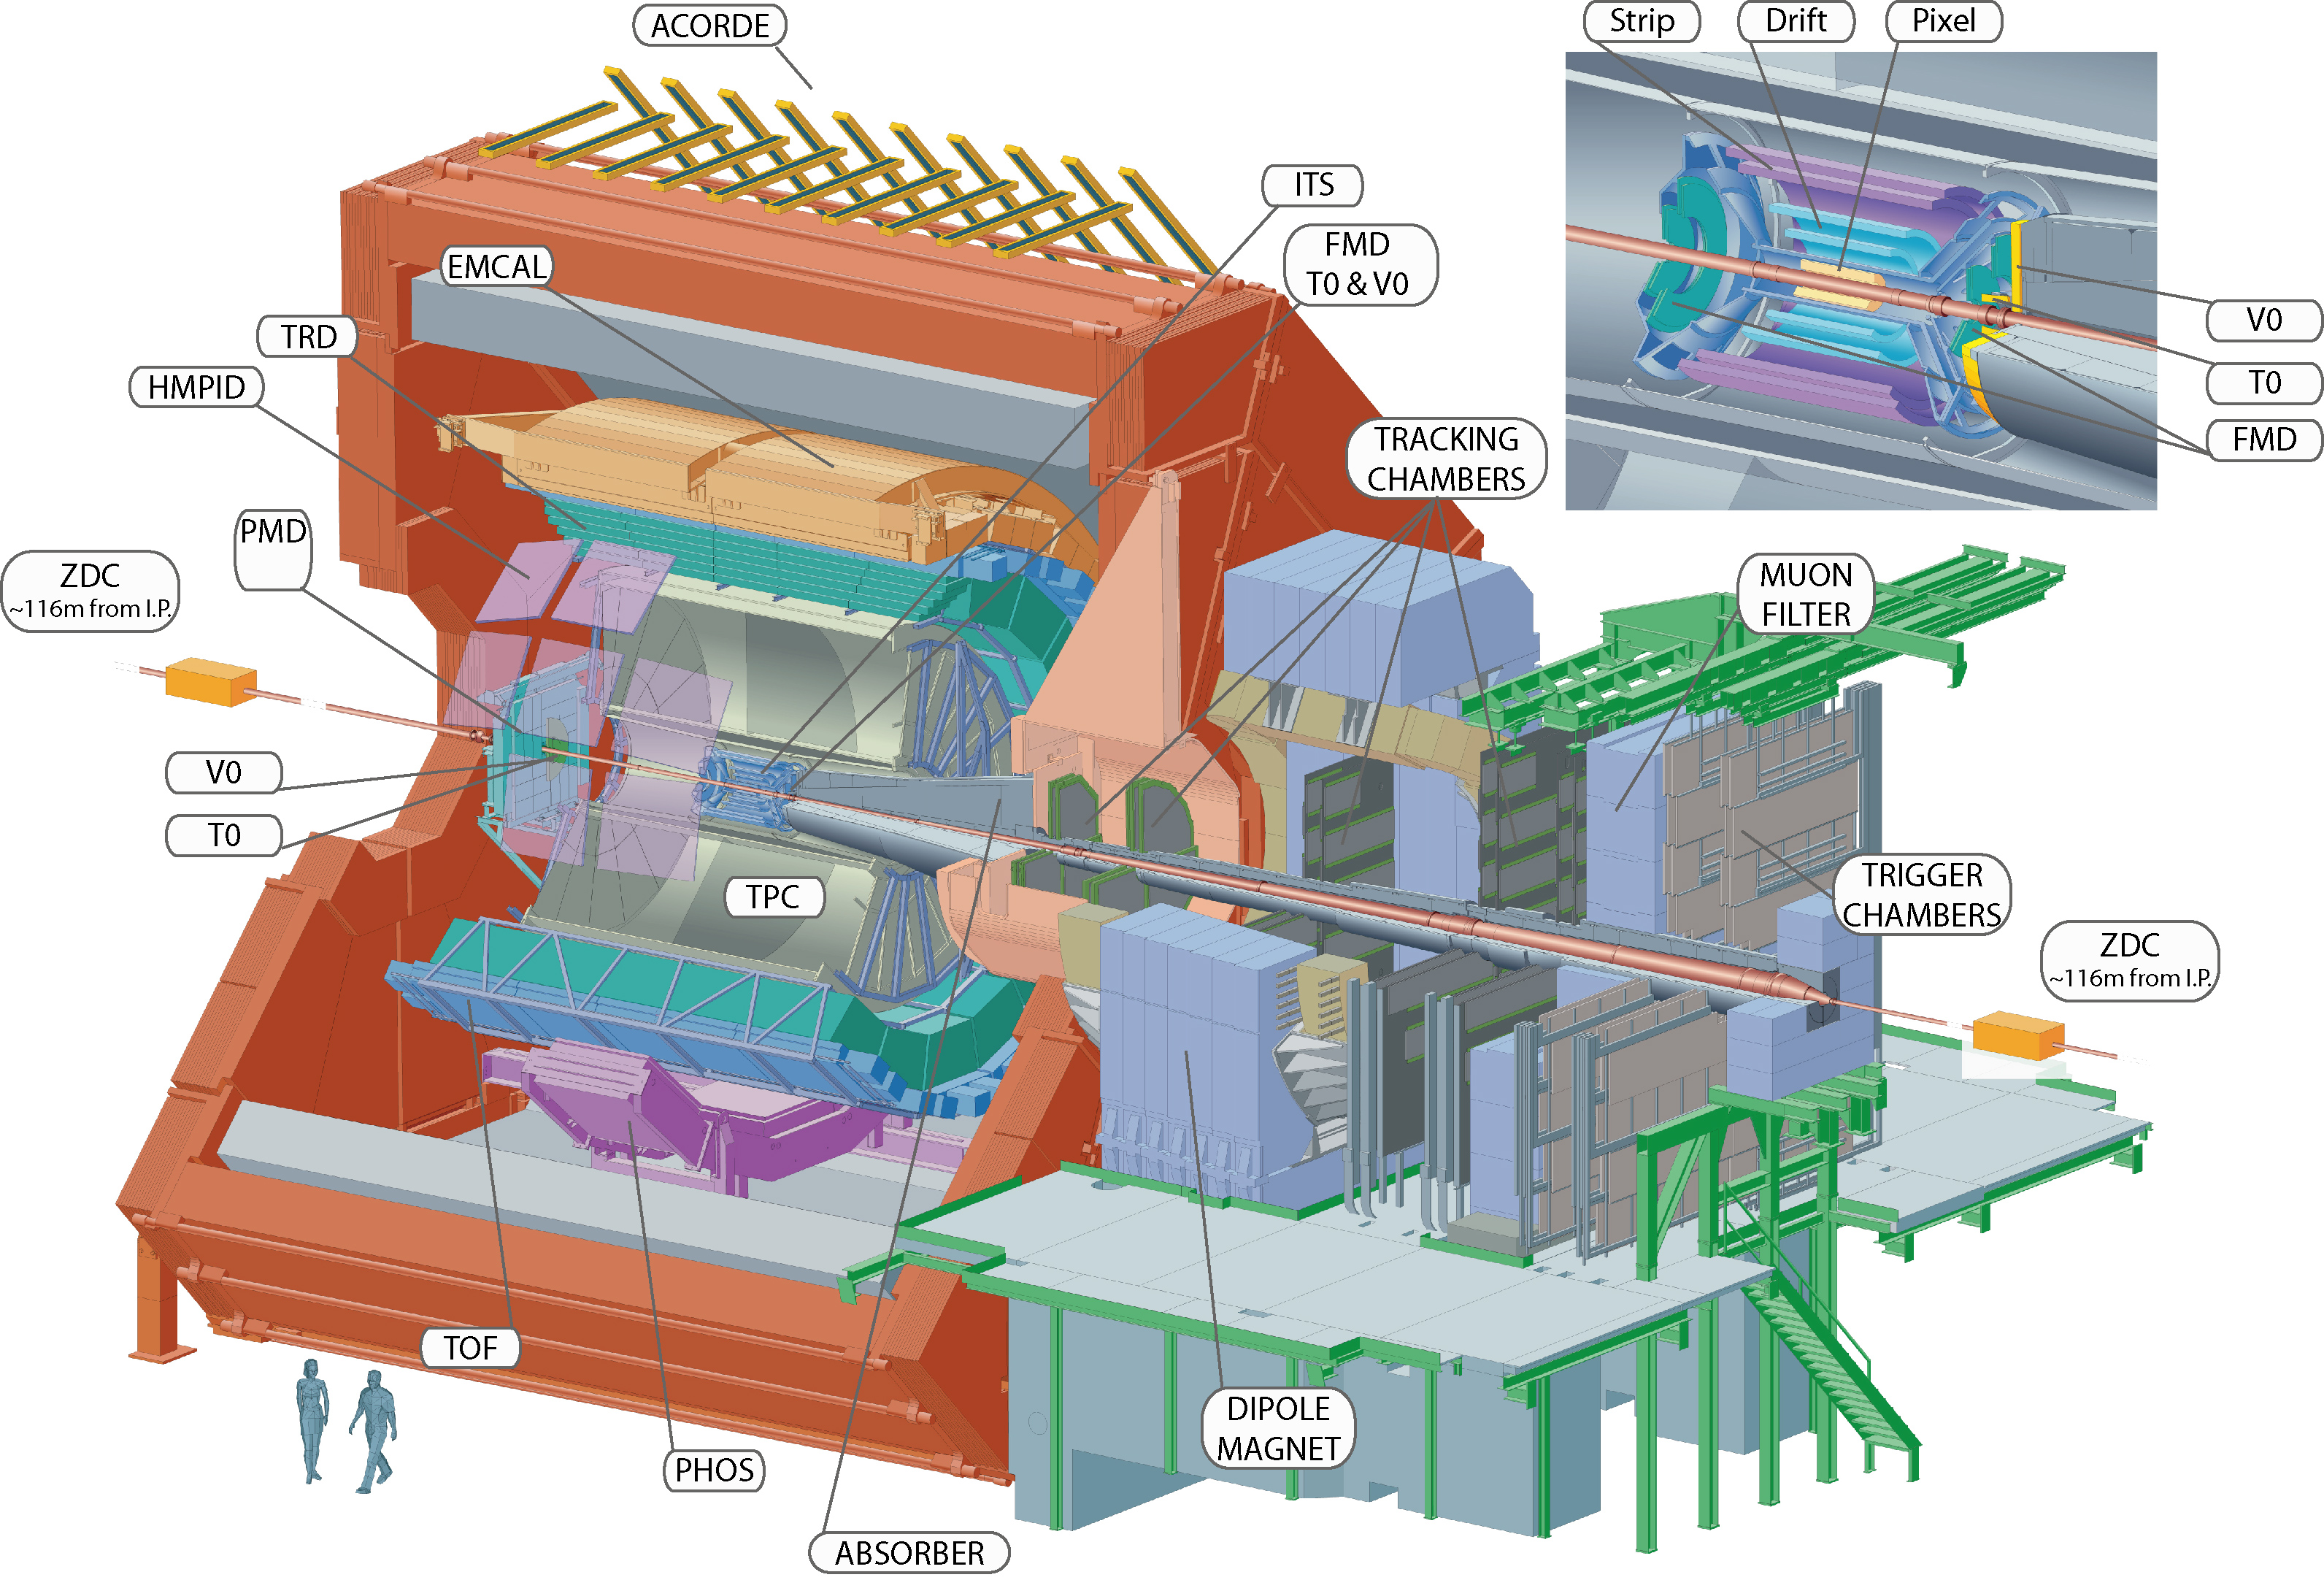
\includegraphics[width=\linewidth]{img/alice_schematics}
 \end{tikzfigure}
\end{minipage}
%
\begin{minipage}[t]{0.48\colwidth}
\begin{itemize}
\item Important features
\begin{itemize}
\item \textbf{PID}
(e, $\mu$, $\pi$, K, p, d, ${}^3$He)
\item \textbf{low-momentum tracking} ($\pt > 0.15$~\GeVc)
\end{itemize}
\item \textbf{D mesons} via hadronic decays (ITS, TPC, TOF)
\begin{itemize}
\item PID, topological cuts
\item invariant mass analysis
\end{itemize}
\end{itemize}
\end{minipage}

\begin{itemize}
\item \textbf{Jet reconstruction} using \antikt\ algorithm
\begin{itemize}
\item \textcolor{ForestGreen}{charged constituents} (ITS, TPC) $\rightarrow$ \emph{charged jets} (this analysis)
\item add \textcolor{NavyBlue}{neutral constituents} (EMCal, DCal) $\rightarrow$ \emph{full jets} 
\end{itemize}
\end{itemize}
}

\column{.29}
\block{Reconstruction Efficiency}{
\begin{minipage}[t]{0.44\colwidth}
\begin{tikzfigure}[Prompt vs. non-prompt.\par]
     \label{fig:Efficiency_QM17}
    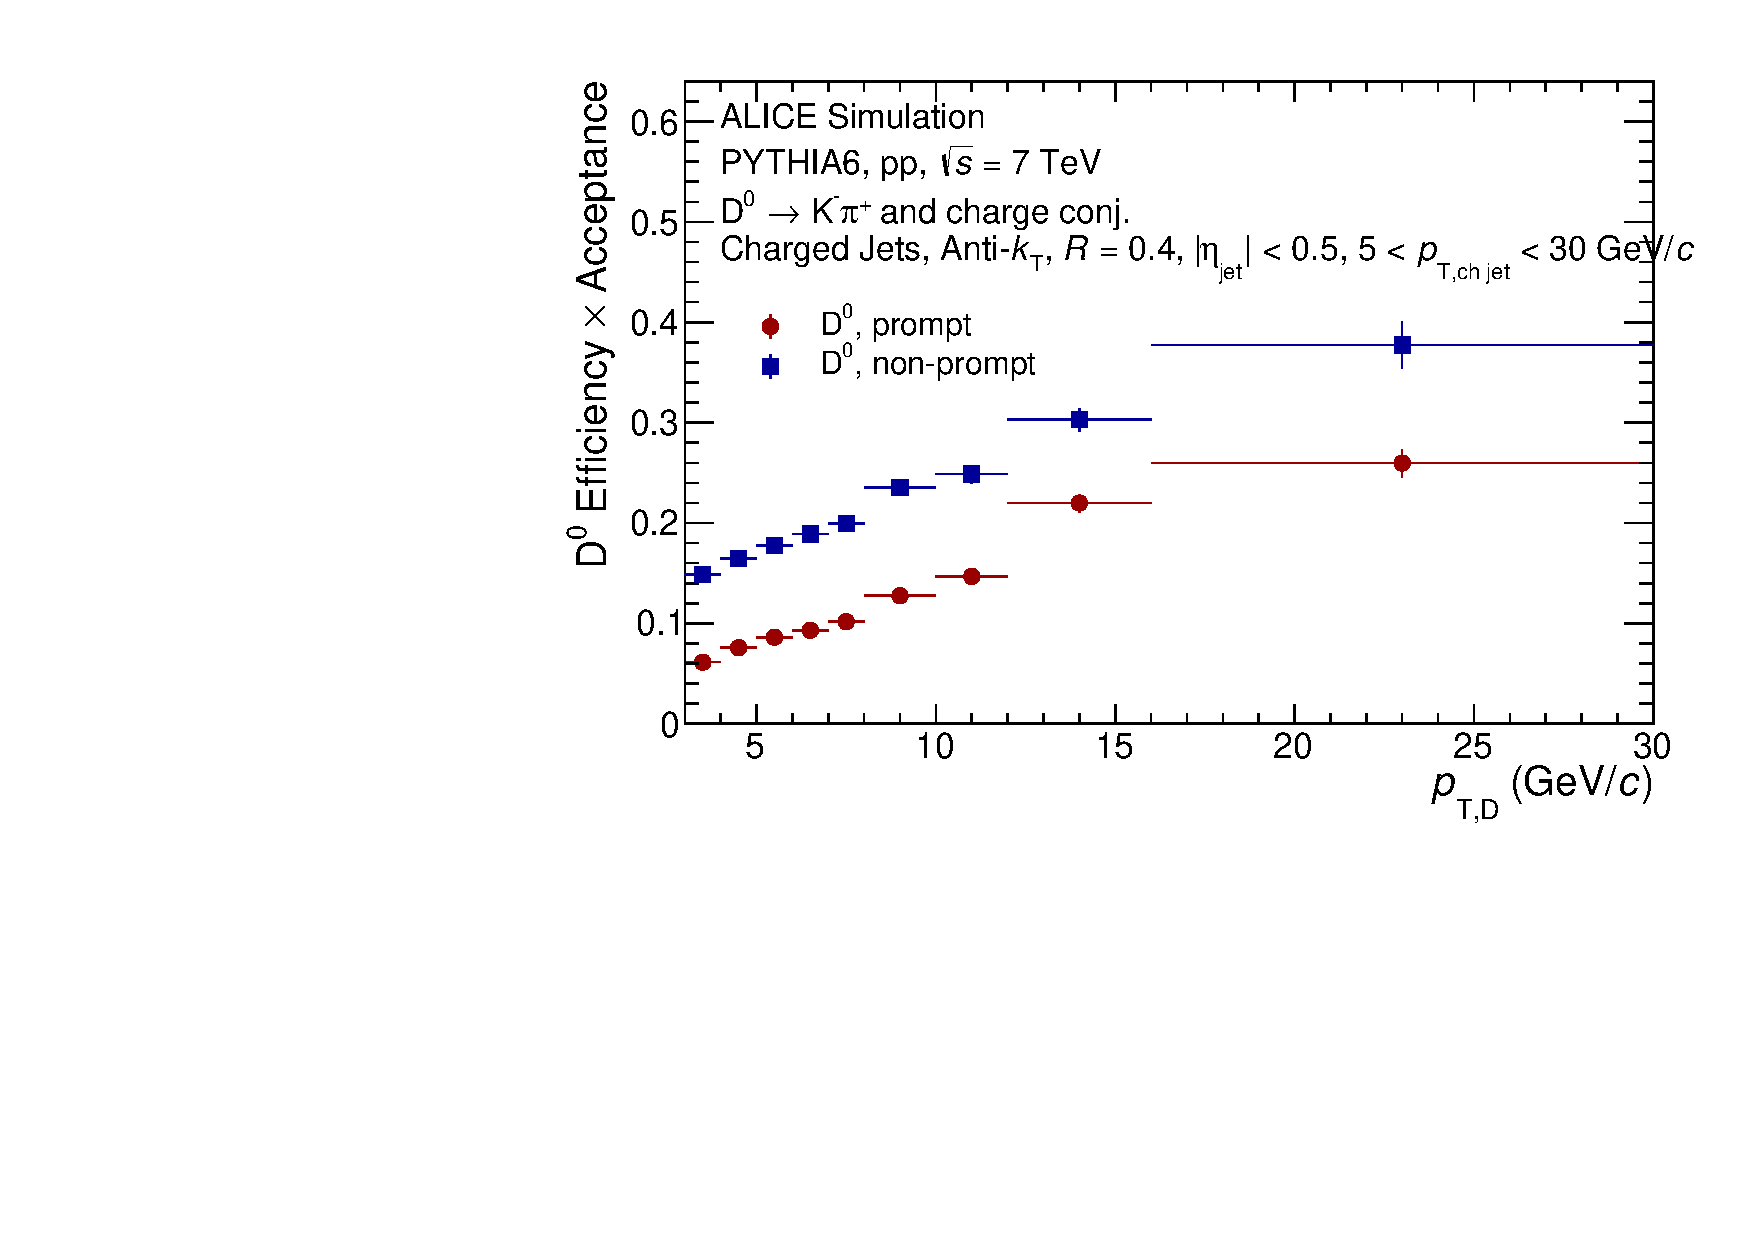
\includegraphics[width=\linewidth]{img/Efficiency_QM17}
 \end{tikzfigure} 
\end{minipage}
%
\begin{minipage}[t]{0.44\colwidth}
\begin{tikzfigure}[Efficiency vs. \ptchjet\par]
     \label{fig:HQ16_Simulation_EfficiencyVsDPt}
    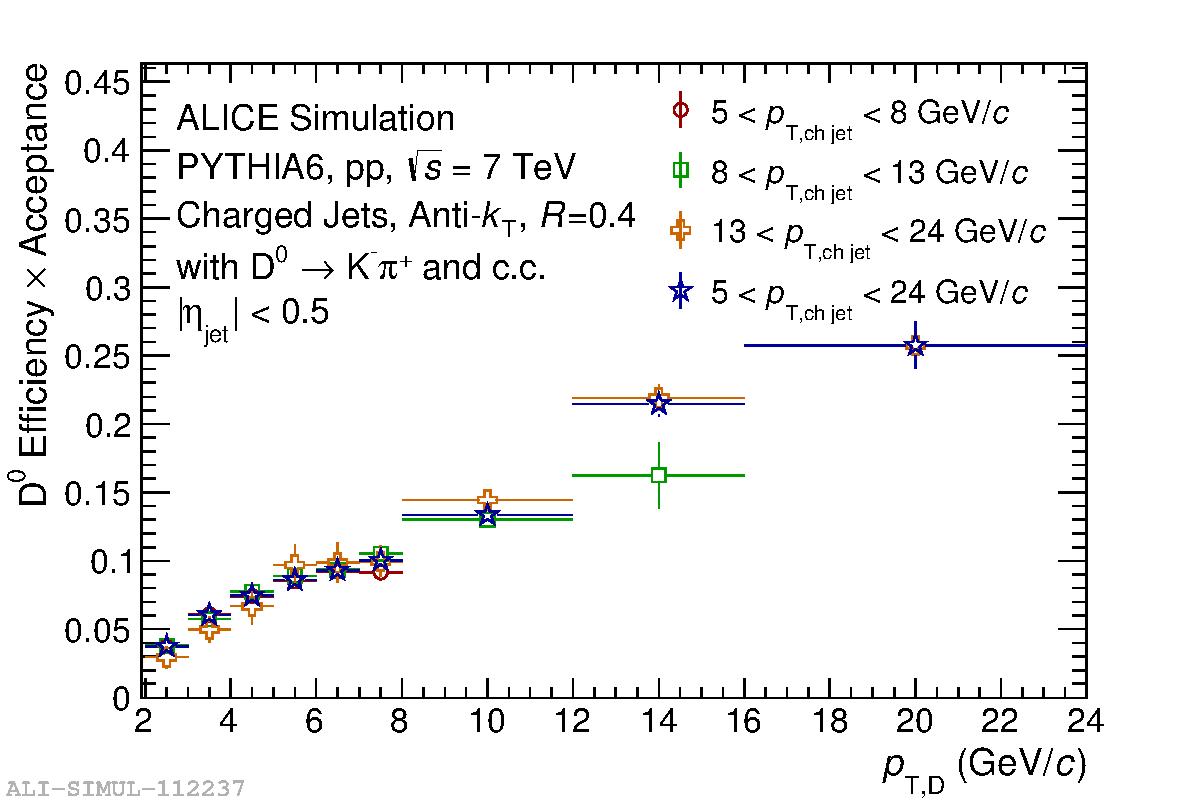
\includegraphics[width=\linewidth]{img/HQ16_Simulation_EfficiencyVsDPt}
 \end{tikzfigure}
\end{minipage}
\begin{itemize}
\item Weak or no dependence on the jet \pt\ $\rightarrow$ simplify corrections and reduces systematics
\item Higher non-prompt efficiency (topological cuts) $\rightarrow$ bias in the relative contributions of the reconstructed yields
\end{itemize}
}

\end{columns}

\begin{columns}
\column{.58}
\block{\Dzero-Jet \pt-Differential Cross Section}{
\begin{minipage}[t]{0.60\colwidth}
\begin{tikzfigure}[Prompt \Dzero-jet \pt-differential cross section in \pp\ collisions at $\s=7$~TeV]
     \label{fig:D0JetCrossSection_pp7TeV}
    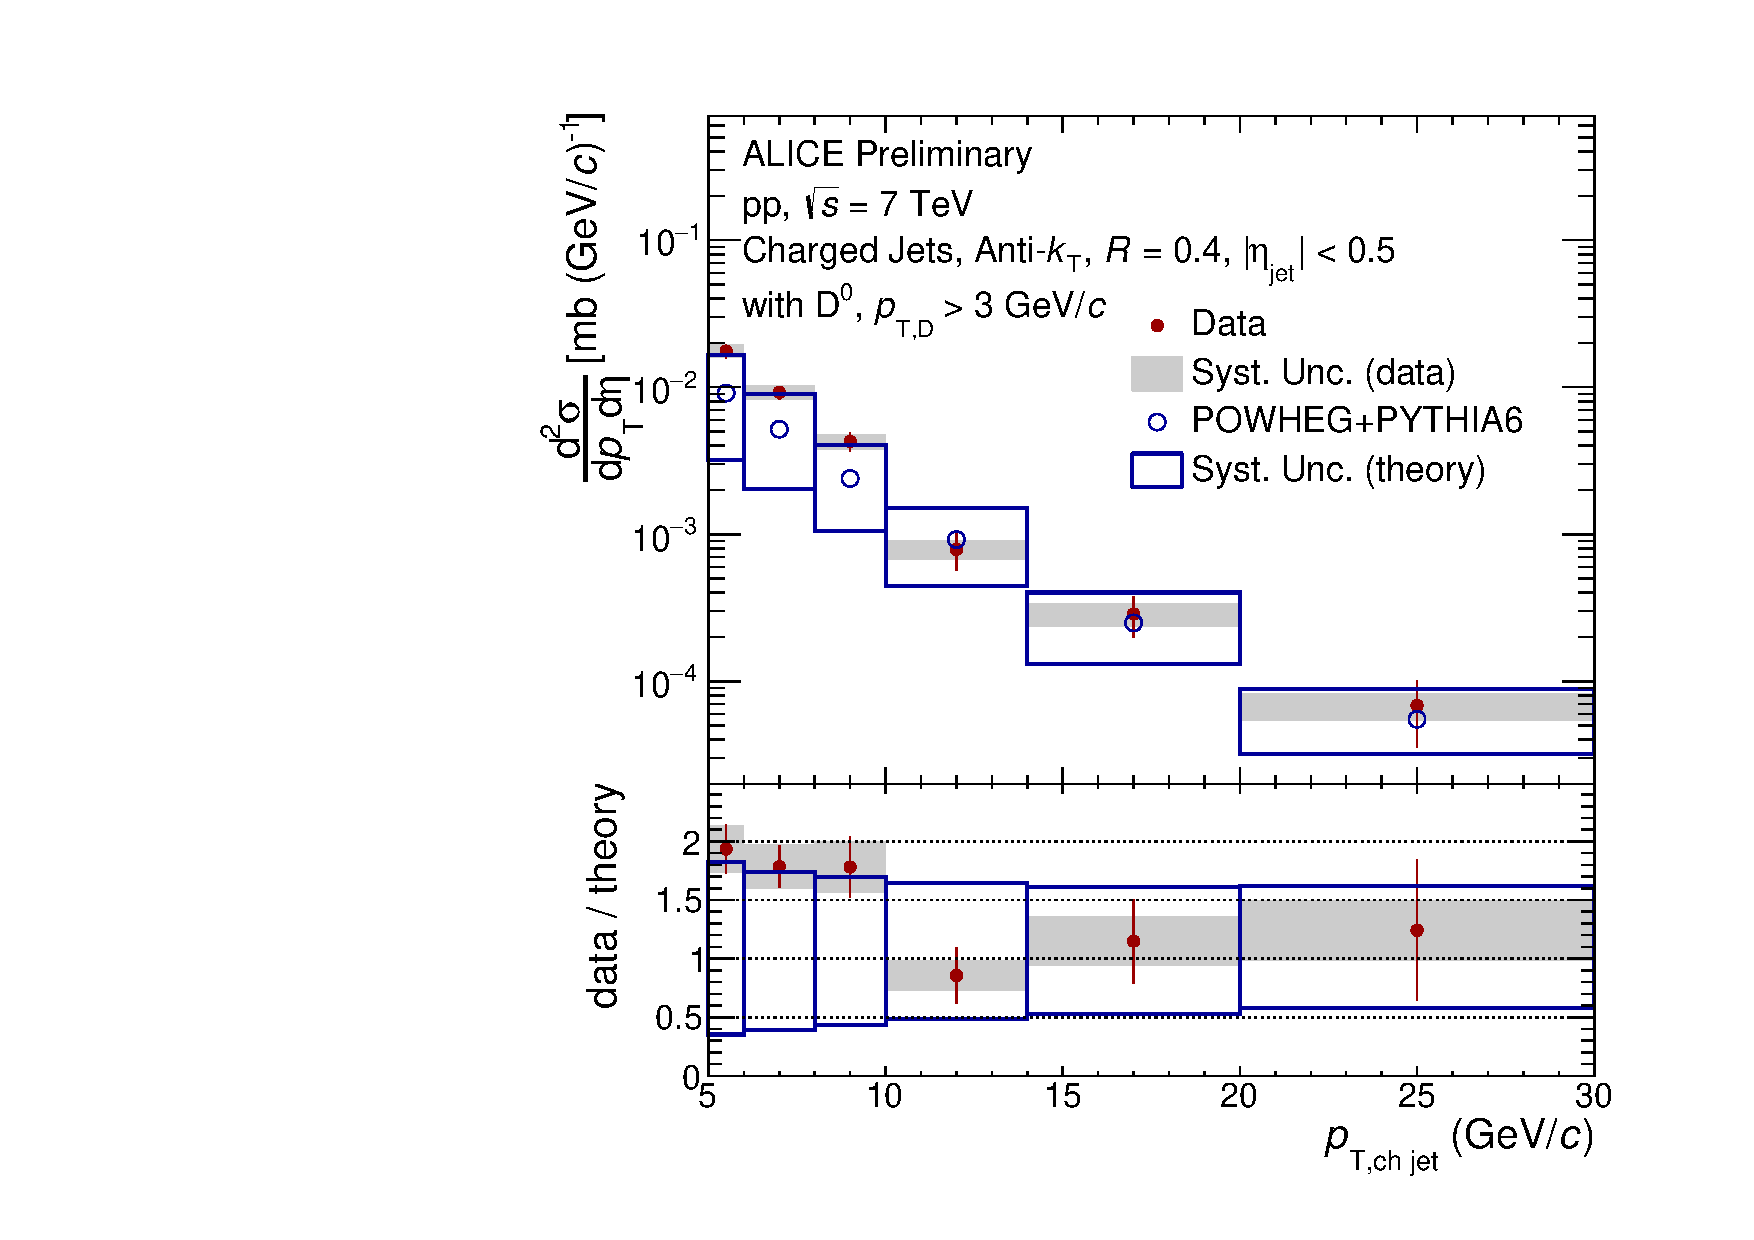
\includegraphics[width=.9\linewidth]{img/D0JetCrossSection_pp7TeV}
 \end{tikzfigure}
\end{minipage}
\begin{minipage}[t]{0.40\colwidth}
bla bla
\end{minipage}
}
\column{.42}

\block{Signal Extraction}{
\begin{tikzfigure}[Top: invariant mass distributions; bottom: jet \pt\ distributions from signal region and side bands.\par]
     \label{fig:SideBandInvMass_QM17}
    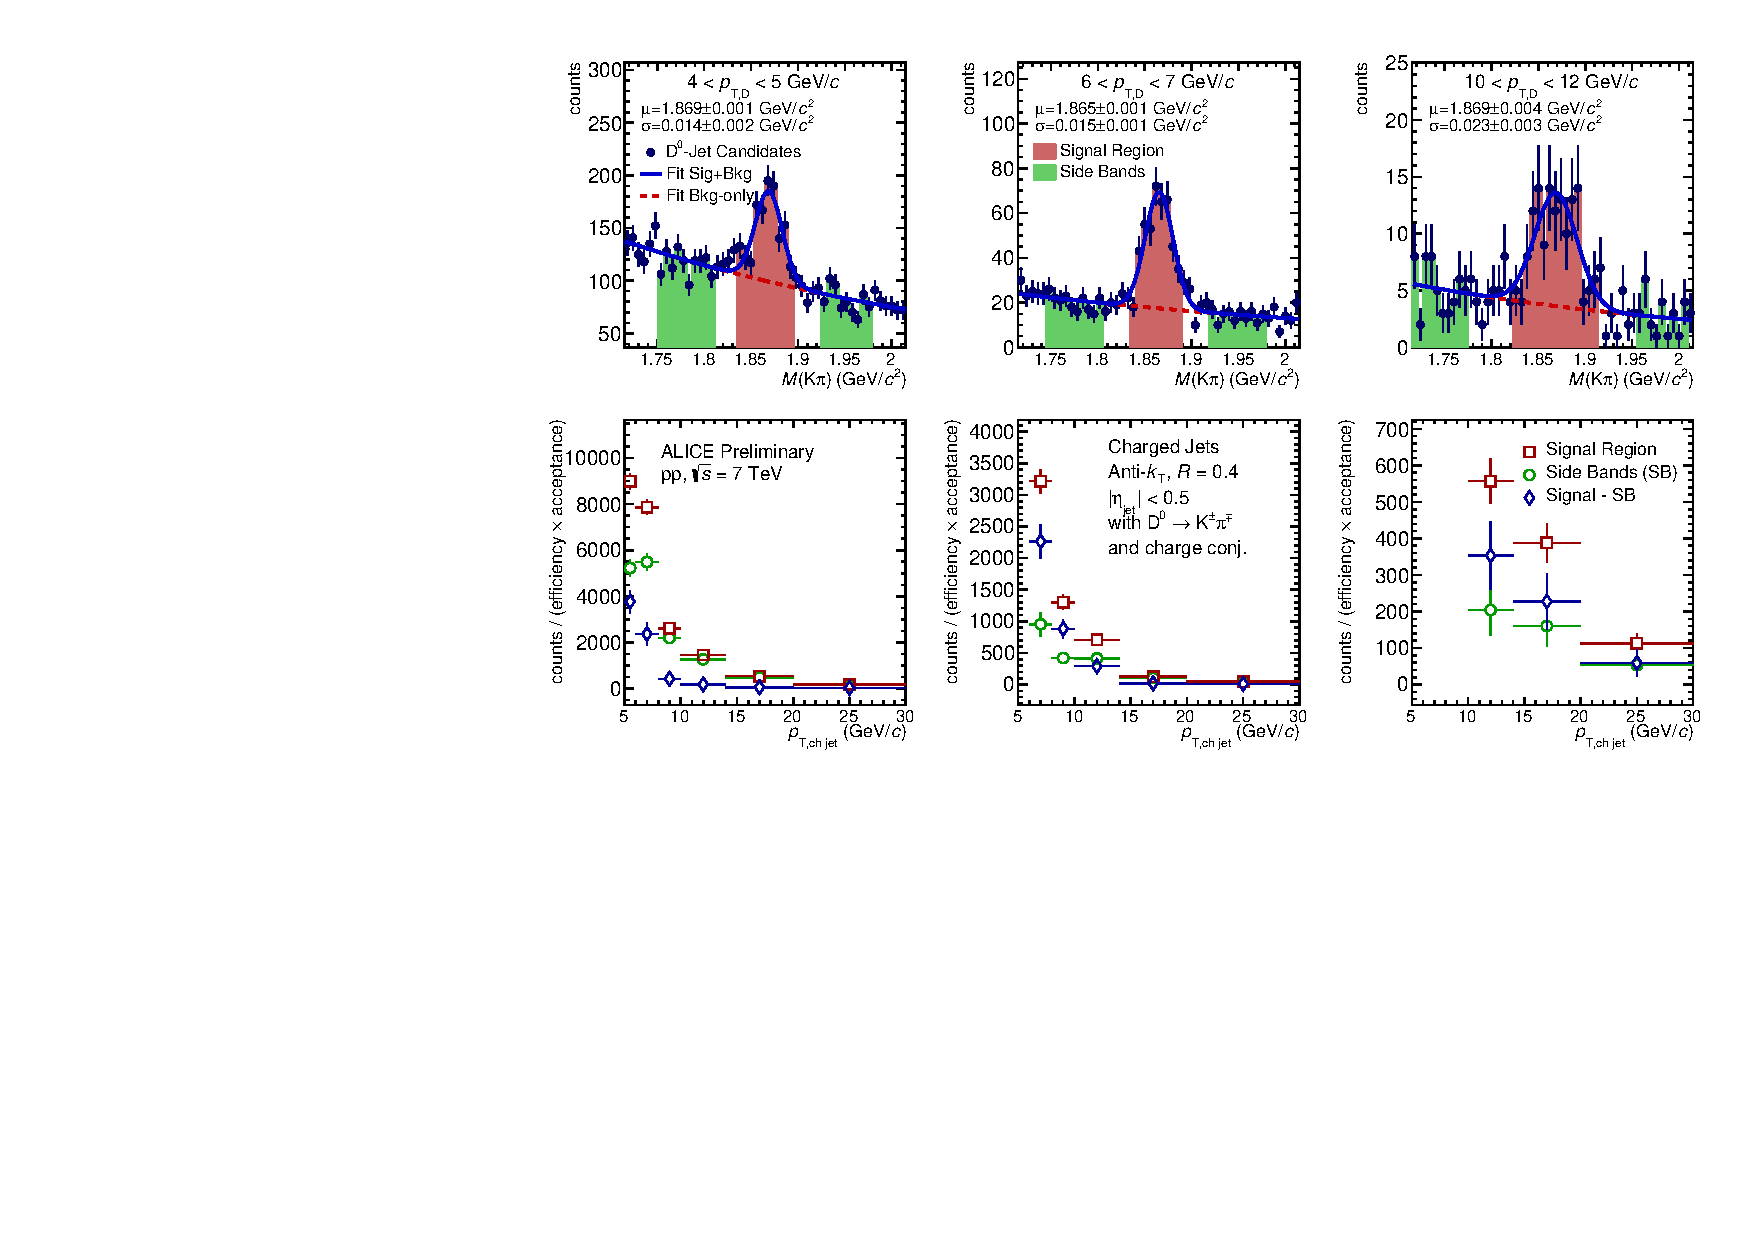
\includegraphics[width=.9\colwidth]{img/SideBandInvMass_QM17}
 \end{tikzfigure}
\begin{itemize}
\item 
\end{itemize}
}
\end{columns}

\begin{columns}
\column{.65}
\block{Jet Momentum Resolution}{

\begin{minipage}[t]{0.4\colwidth}
\begin{tikzfigure}[Prompt \Dzero-jet \pt-differential cross section in \pp\ collisions at $\s=7$~TeV]
     \label{fig:HQ16_Simulation_EnergyScaleShift}
    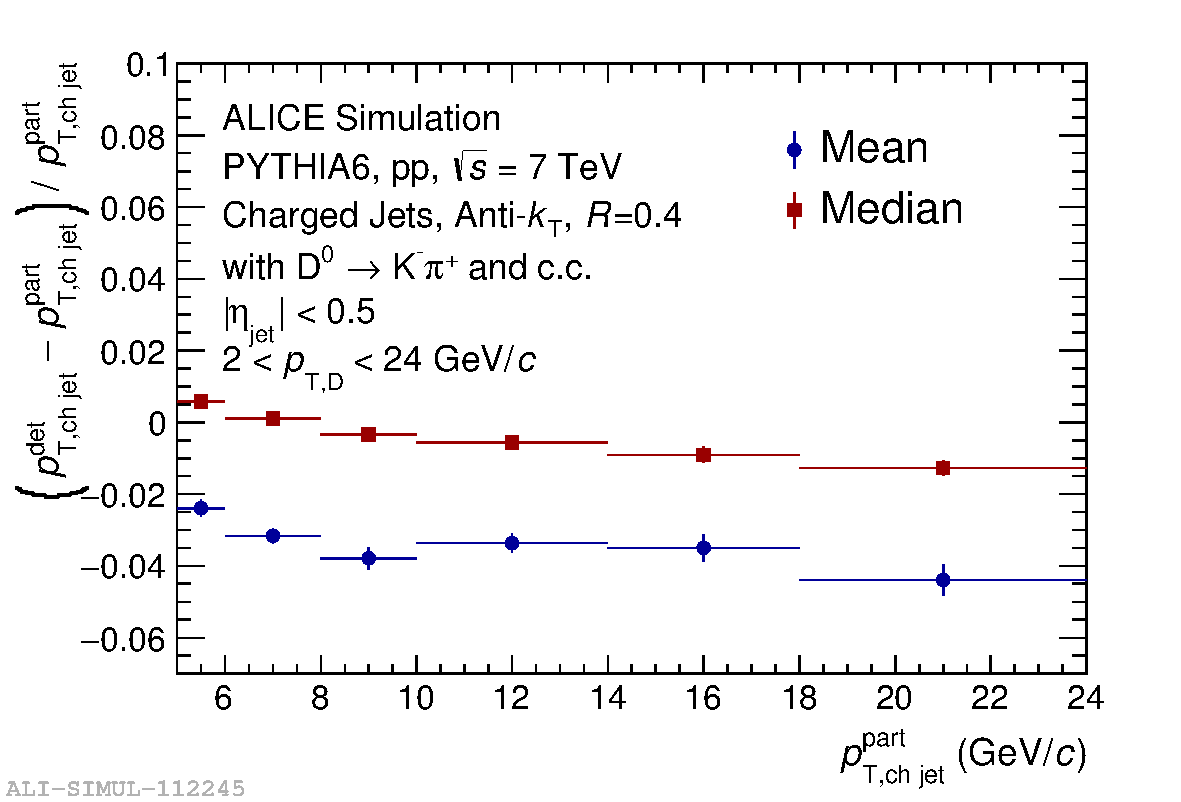
\includegraphics[width=.9\linewidth]{img/HQ16_Simulation_EnergyScaleShift}
 \end{tikzfigure}
\begin{tikzfigure}[Prompt \Dzero-jet \pt-differential cross section in \pp\ collisions at $\s=7$~TeV]
     \label{fig:HQ16_Simulation_Resolution}
    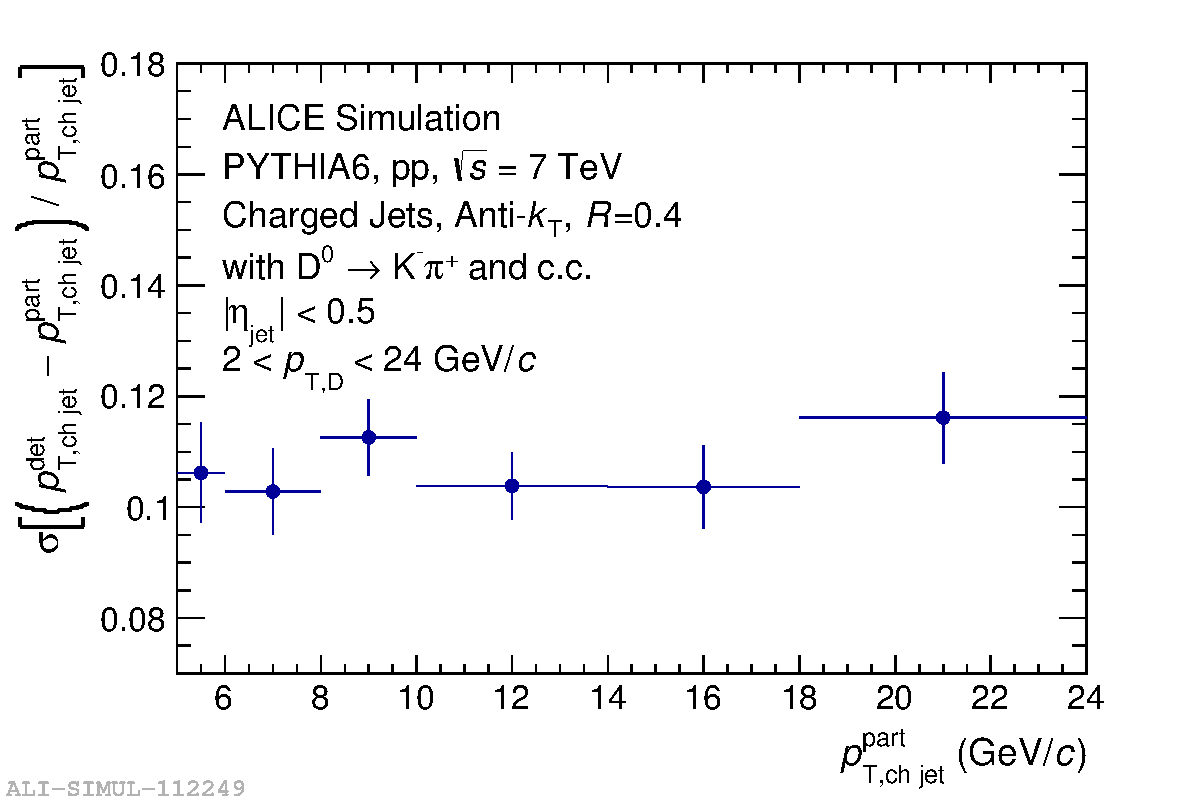
\includegraphics[width=.9\linewidth]{img/HQ16_Simulation_Resolution}
 \end{tikzfigure}
\end{minipage}%
%
\begin{adjustbox}{valign=t}
\begin{minipage}[t]{0.6\colwidth}
\begin{tikzfigure}[Prompt \Dzero-jet \pt-differential cross section in \pp\ collisions at $\s=7$~TeV]
     \label{fig:HQ16_Simulation_DetectorResponse}
    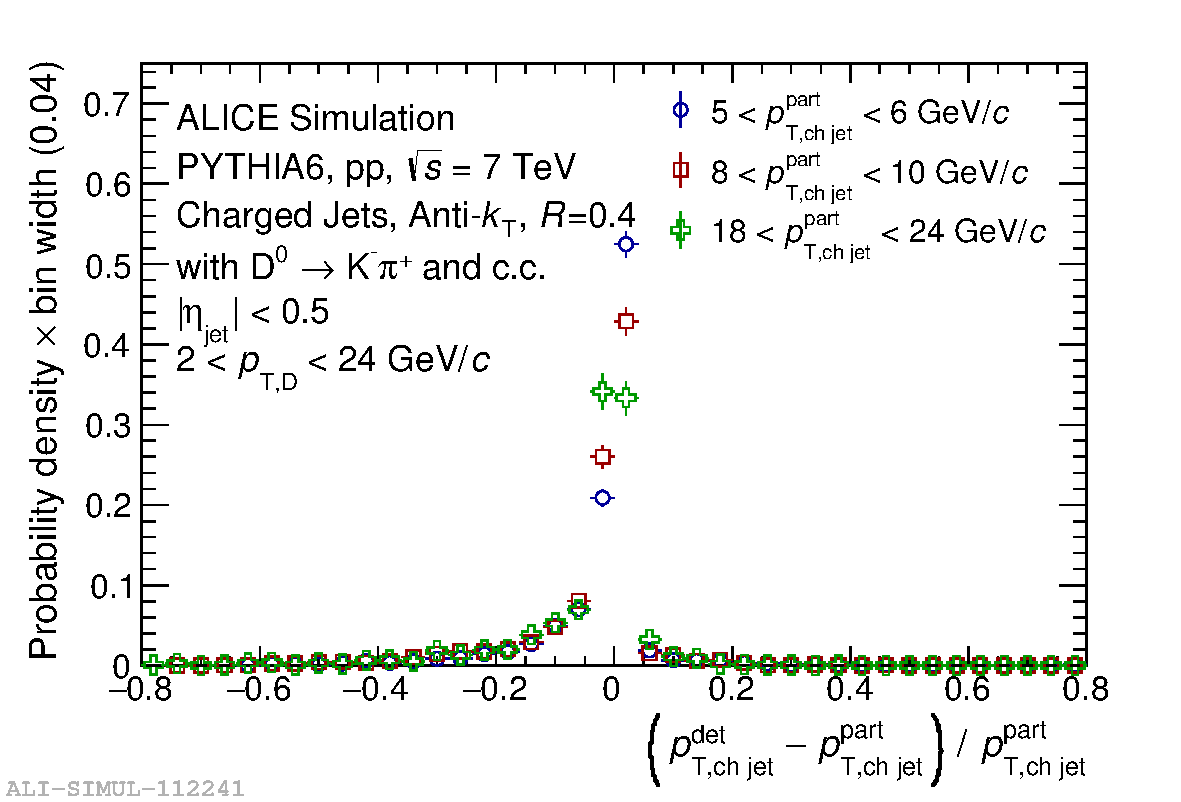
\includegraphics[width=.9\linewidth]{img/HQ16_Simulation_DetectorResponse}
 \end{tikzfigure}
\end{minipage}
\end{adjustbox}

}
\column{.35}

\block{B Feed-Down Subtraction}{
\begin{minipage}[t]{0.45\colwidth}
\begin{tikzfigure}[Prompt \Dzero-jet \pt-differential cross section in \pp\ collisions at $\s=7$~TeV]
     \label{fig:BFeedDown_QM17}
    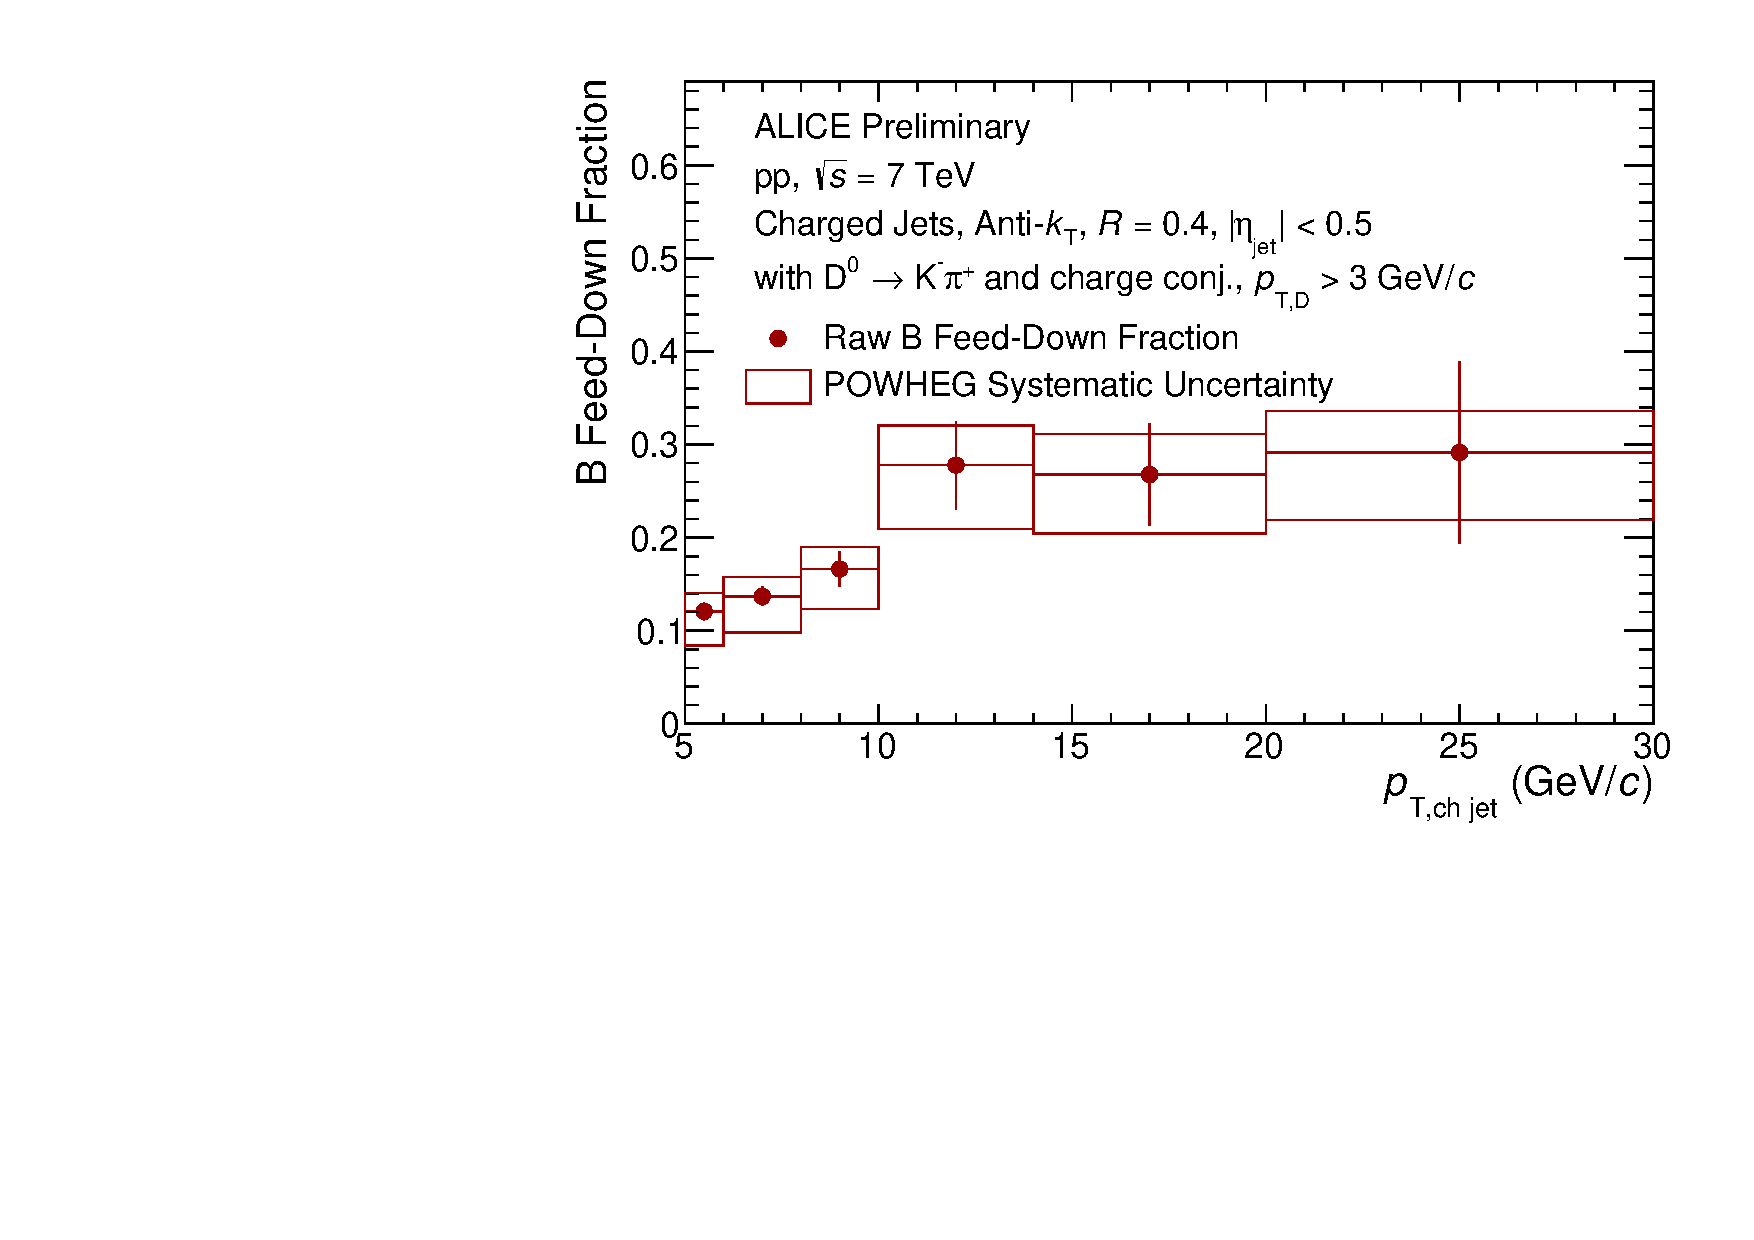
\includegraphics[width=.9\linewidth]{img/BFeedDown_QM17}
 \end{tikzfigure}
\end{minipage}
\begin{minipage}[t]{0.45\colwidth}
bla bla
\end{minipage}
}

\block{Conclusions}{
\begin{tikzfigure}[Prompt \Dzero-jet \pt-differential cross section in \pp\ collisions at $\s=7$~TeV]
     \label{fig:Uncertainties_QM17}
    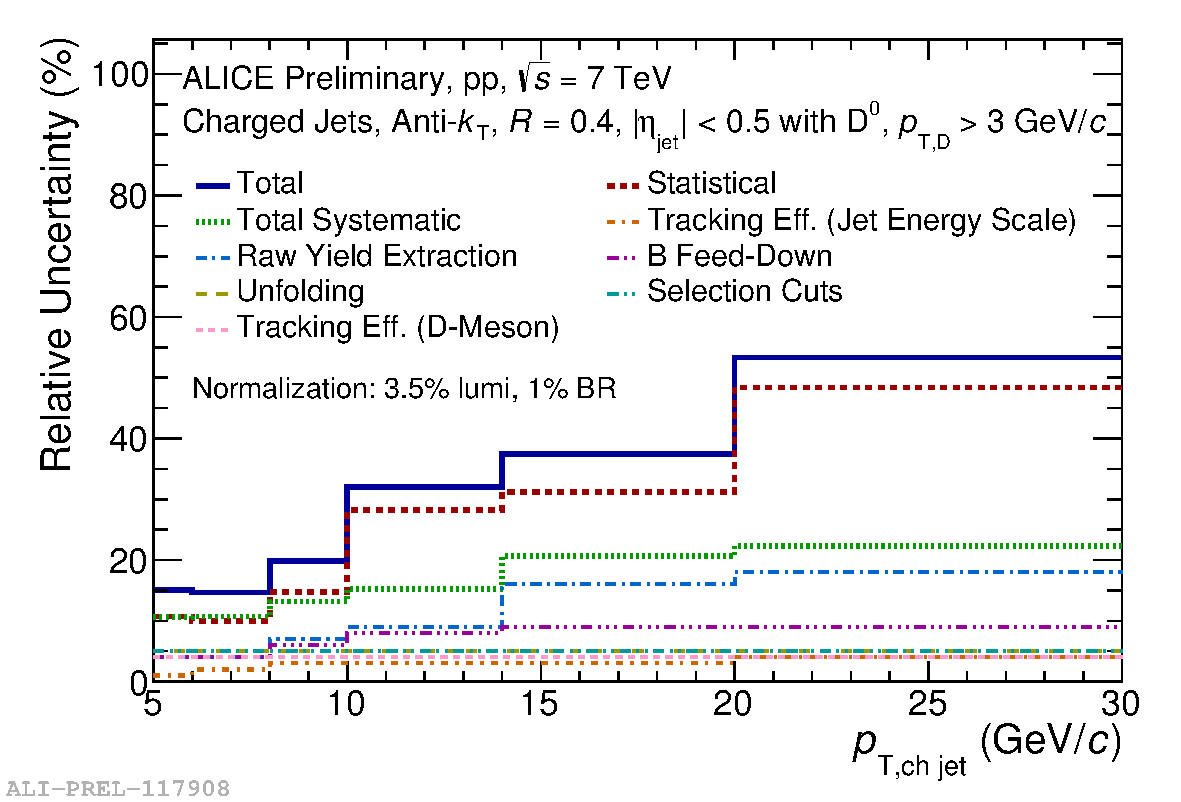
\includegraphics[width=.5\colwidth]{img/Uncertainties_QM17}
 \end{tikzfigure}
}
\end{columns}

\end{document}
